\documentclass{standalone}
\input{feynman_settings}

\begin{document}

\raisebox{+2.6ex}{\Large$\partial_t$}
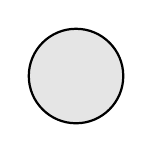
\begin{tikzpicture}
\vspace{1cm}
\draw[thick, fill = gray!20] circle(0.6);
\end{tikzpicture}
\raisebox{+2.6ex}{\large{\hspace{5pt} $=$ \hspace{5pt}} \huge $\frac{1}{2}$} 

\raisebox{-2ex}{
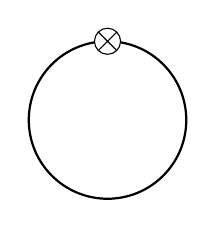
\begin{tikzpicture}[cross/.style={path picture={ 
\draw[black]
(path picture bounding box.south east) -- (path picture bounding box.north west) (path picture bounding box.south west) -- (path picture bounding box.north east);
}}]
\draw[thick] circle(1);
\node [draw, fill = white, circle,cross,minimum width= 0.1 cm] at (0,1){}; 
\end{tikzpicture}
}
 
\end{document}